% !TeX document-id = {87432cc9-c386-48dc-9558-b3c42a74a150}
% !TEX encoding = UTF-8
% !TEX TS-program = pdflatex
% !TEX spellcheck = it-IT
%% !TEX root = 
% !BIB TS-program = biber
% Comandi speciali (o righe magiche) trattati come commenti da Latex ma non da 
%editor come Texstudio e Texshop, che si impostano di conseguenza. In ordine:
% dichiara la codifica dei caratteri con cui impostare l'editor (bisogna 
%comunque caricare inputenc con la stessa codifica)
% dichiara il motore di composizione (pdflatex o lualatex)
% attiva il controllo ortografico della lingua del documento
% dichiara la condizione di file principale e di file secondario nei documenti 
%suddivisi in più file
% imposta biber come motore bibliografico

\documentclass[9pt]{extarticle}


% ------------------------------------------------------------------------------
% Packages
% ------------------------------------------------------------------------------
\usepackage[utf8]{inputenc}
\usepackage{graphicx}
\usepackage{amsmath}
\usepackage{amssymb}
\usepackage{amsthm}
\usepackage{hyperref}
\usepackage{titlesec}
\usepackage{parskip}
\usepackage{float}
\usepackage{booktabs}
\usepackage{caption}
\usepackage{blindtext}
\usepackage[table,xcdraw]{xcolor}
\usepackage{enumitem}
% Define a new counter for functional requirements
\newcounter{rf}
\newcommand{\FR}{\refstepcounter{rf}\textbf{FR\therf: }}
% Define a new counter for non-functional requirements
\newcounter{nonfunc}
\newcommand{\NONFUNC}{\refstepcounter{nonfunc}\textbf{NFR\thenonfunc: }}

% ------------------------------------------------------------------------------
% Page setup
% ------------------------------------------------------------------------------
\usepackage{geometry} 
\geometry{a4paper, margin=1in, twoside}
\usepackage{setspace}
\setstretch{1.2}  % Adjust the number as needed
%\doublespacing


% ------------------------------------------------------------------------------
% Referencing
% ------------------------------------------------------------------------------
\usepackage[
	backend=biber,
	citestyle=authoryear,
	bibstyle=authoryear,
	maxcitenames=2,
	maxbibnames=99]{biblatex}
%\addbibresource{references.bib}
%\DeclareNameAlias{sortname}{family-given}
%\setlength\bibitemsep{1em}

% ------------------------------------------------------------------------------
% Code listings
% ------------------------------------------------------------------------------
\usepackage{listings}
\usepackage{xcolor}
\lstdefinestyle{matlabcode}{
	backgroundcolor=\color{gray!10},   
	commentstyle=\color{green!50!black},
	keywordstyle=\color{blue},
	stringstyle=\color{magenta},
	basicstyle=\linespread{1}\footnotesize\ttfamily,
	numberstyle=\tiny,
	breakatwhitespace=false,         
	breaklines=true,                 
	captionpos=t,   
	frame=single,
	keepspaces=true,         
	language=matlab,        
	numbers=none,             
	numbersep=5pt,                  
	showspaces=false,                
	showstringspaces=false,
	showtabs=false,                  
	tabsize=2,
	aboveskip=1em,
	belowskip=1em,
	belowcaptionskip=12pt
}

% ------------------------------------------------------------------------------
% Headers and footers
% ------------------------------------------------------------------------------	
\usepackage{fancyhdr}
\pagestyle{fancy}   
\setlength{\headheight}{14.5pt}
\renewcommand{\headrulewidth}{0.3pt}
%\renewcommand{\chaptermark}[1]{\markboth{\chaptername\ \thechapter.\ #1}{}}
\renewcommand{\sectionmark}[1]{\markright{\thesection.\ #1}}   
\fancyhead[LE,RO]{\rightmark}
\fancyhead[LO,RE]{\leftmark}

% ------------------------------------------------------------------------------
% Title page
% ------------------------------------------------------------------------------

\newcommand{\name}{Togni Roberto}
\newcommand{\projecttitle}{EvenTrento}
\newcommand{\course}{Ingegneria del Software}
\newcommand{\customtitle}{
	\vspace*{1cm}
	\begin{center}
		
\includegraphics[width = 7cm]{images/logo_rosso} \\
		\vspace{1cm}
	\end{center}
	\LARGE{Progetto:}
	\begin{center}
%		\vspace{2cm}
		\textbf{\Huge{\projecttitle}} \\
	\end{center}
	\LARGE{Titolo del documento:}
	\begin{center}
%		\vspace{1cm}
		\textbf{\Huge Descrizione di Progetto} \\
	\end{center}
	\LARGE{Autore:}
	\begin{center}
		%		\vspace{1cm}
		\textbf{\name} \\
	\end{center}
	\vspace{1cm}
	Document Info:
	
	\begingroup
	\setlength{\tabcolsep}{10pt} % Default value: 6pt
	\renewcommand{\arraystretch}{1.5}
	
	\begin{table}[!htb]
		\begin{tabular}{lllll}
			\cline{1-4}
			\cellcolor[HTML]{13315C}{\color[HTML]{FFFFFF} Doc. Name}                         & D1-EvenTrentoDescrizioneProgetto & \multicolumn{1}{l|}{\cellcolor[HTML]{13315C}{\color[HTML]{FFFFFF} Doc. Number}} & \multicolumn{1}{l|}{D1 V0.1} &  \\ \cline{1-4}
			\multicolumn{1}{|l|}{\cellcolor[HTML]{13315C}{\color[HTML]{FFFFFF} Description}} & \multicolumn{3}{l|}{Documento di analisi dei requisiti funzionali, non funzionali e front-end}                                                    &  \\ \cline{1-4}
			&                                  &                                                                                 &                              &  \\
			&                                  &                                                                                 &                              &  \\
		\end{tabular}
	\end{table}
	
	\endgroup
	
	\begin{center}
		\vfill 
		\textbf{\Large Dipartimento di Ingegneria e Scienza dell'Informazione}
		\vspace{1cm}
	\end{center}
	\newpage
	\pagenumbering{roman}
	\setcounter{page}{0}
}

% ------------------------------------------------------------------------------
% Theorem enivornments
% ------------------------------------------------------------------------------
%\newtheorem{theorem}{Theorem}[chapter]
%\newtheorem{definition}{Definition}[chapter]
%\newtheorem{corollary}{Corollary}[theorem]
%\newtheorem{lemma}[theorem]{Lemma}

\newtheoremstyle{break}%
    {}{}%
    {}{}%
    {\bfseries}{}% % Note that final punctuation is omitted.
    {\newline}{}
\theoremstyle{break}
%\newtheorem{example}{Example}[chapter]



% ------------------------------------------------------------------------------
% Document
% ------------------------------------------------------------------------------


\begin{document}
\customtitle



% TODO add chapters
\tableofcontents
\newpage

\section{Scopo del Documento}

Il presente documento ha lo scopo di riportare le informazioni riguardanti lo
sviluppo di una parte dell'applicazione EvenTrento. Partendo dalle user stories,
il documento presenta un walk-throgh delle funzionalità effettivemente
implementate, con un focus sull'interazione dell'utente con queste ultime.
Prosegue dunque con la descrizione delle web APIs del'applicazione, nonché
della modalità di sviluppo collaborativo, del database e del testing delle varie
funzionalità.
Infine, viene presentato il front-end realizzato, accompagnato da una
descrizione della modalità di deployment utilizzata.

\newpage

\section{User Stories}

Le seguenti tabelle raccolgono una sere di User Stories divise in diverse epiche. Ad ogni user story è associata una priorità (ad un numero più piccolo corrisponde una priorità maggiore) rappresentante l'importanza della funzionalità in questione per l'operatività del sistema.

	
\begin{table}[!htb]
	\centering
	\renewcommand{\arraystretch}{1.7} % Increased vertical spacing
	\begin{tabular}{clp{7cm}l} % Use 'p{7cm}' for the User Story column
		\toprule
		\rowcolor{gray!20}
		\multicolumn{4}{c}{\textbf{Profilo}}\\ \midrule
		\rowcolor{gray!20}
		Id & Nome & User Story & Priorità \\ \midrule
		A1  & Registrazione  & Come utente, voglio registrarmi per utilizzare il sistema & 1 \\
		A2  & Login & In qualità di utente, devo essere in grado di effettuare il login & 1 \\
		A3  & Visualizzazione profilo & Come utente, devo essere in grado di visualizzare lo storico eventi, le mie informazioni personali, e gli eventi salvati &  2\\
		\bottomrule
	\end{tabular}
	\caption{User stories relative all'epica "profilo".}
	\label{tab:profili}
\end{table}


\begin{table}[!htb]
	\centering
	\renewcommand{\arraystretch}{1.7}
	\begin{tabular}{clp{7cm}l} % Use 'p{7cm}' for the User Story column
		\toprule
		\rowcolor{gray!20}
		\multicolumn{4}{c}{\textbf{Eventi}}\\ \midrule
		\rowcolor{gray!20}
		Id & Nome & User Story & Priorità \\ \midrule
		B1  & Lista eventi            & In qualità di utente, devo essere in grado di scorrere una lista di eventi                                               &  1\\
		B2  & Filtri eventi           & In qualità di utente, devo essere in grado di filtrare gli eventi in base a diversi criteri                                      &  2 \\
		B3  & Creazione evento        & In qualità di organizzatore, devo essere in grado di creare un nuovo evento in un determinato luogo                      &  2 \\
		B4  & Condivisione evento     & In qualità di utente, devo essere in grado di condividere un evento tramite link                                         &  4\\
		B5  & Pagamento               & In qualità di utente, devo essere in grado di effettuare il pagamento per un evento a cui voglio iscrivermi              & 2\\
		B6  & Aggiornamento evento    & In qualità di organizzatore, devo essere in grado di aggiornare la descrizione di un evento                              & 3\\
		B7  & Statistiche evento      & In qualità di organizzatore, devo essere in grado di visualizzare gli iscritti all'evento                                & 4\\
		B8  & Salvataggio evento      & In qualità di utente, devo essere in grado di salvare un evento in modo da poterlo visualizzare nella mia area personale & 3\\
		\bottomrule
	\end{tabular}
	\caption{User stories relative all'epica "eventi".}
	\label{tab:eventi}
\end{table}

\newpage

\begin{table}[!htb]
	\centering
	\renewcommand{\arraystretch}{1.7}
	\begin{tabular}{clp{7cm}l} % Use 'p{7cm}' for the User Story column
		\toprule
		\rowcolor{gray!20}
		\multicolumn{4}{c}{\textbf{Spazi}}\\ \midrule
		\rowcolor{gray!20}
		Id & Nome & User Story & Priorità \\ \midrule
		C1  & Aggiunta spazio  & In qualità di owner, devo essere in grado di pubblicare uno spazio disponibile & 2\\
		C2 & Rimozione spazio & In qualità di owner, devo essere in grado di rimuovere uno spazio esistente & 2\\
		C3 & Visualizzazione spazi & In qualità di organizzatore, devo essere in grado di visualizzare gli spazi disponibili & 3\\
		\bottomrule
	\end{tabular}
	\caption{User stories relative all'epica "spazi".}
	\label{tab:spazi}
\end{table}



\begin{table}[!htb]
	\centering
	\renewcommand{\arraystretch}{1.7}
	\begin{tabular}{clp{7cm}l} % Use 'p{7cm}' for the User Story column
		\toprule
		\rowcolor{gray!20}
		\multicolumn{4}{c}{\textbf{Mappa}}\\ \midrule
		\rowcolor{gray!20}
		Id & Nome & User Story & Priorità \\ \midrule
		D1  & Esplorazione mappa      & In qualità di utente, devo essere in grado di muovermi nella mappa per visualizzare gli eventi                           & 1 \\
%		D2  & Aggiunta luogo          & In qualità di owner, devo essere in grado di aggiungere un nuovo luogo alla mappa                                        & \\
		\bottomrule
	\end{tabular}
	\caption{User stories relative all'epica "mappa".}
	\label{tab:mappa}
\end{table}

\newpage

\section{User Flow}

Di seguito sono riportati i diagrammi di flusso rappresentanti gli user flow corrispondenti ad una serie di user stories. La notazione utilizzata nelle descrizioni si riferisce a quella riportata nelle Tabelle \ref{tab:profili}, \ref{tab:eventi}, \ref{tab:spazi} e \ref{tab:mappa}.

\begin{figure}[!htb]
	\centering
	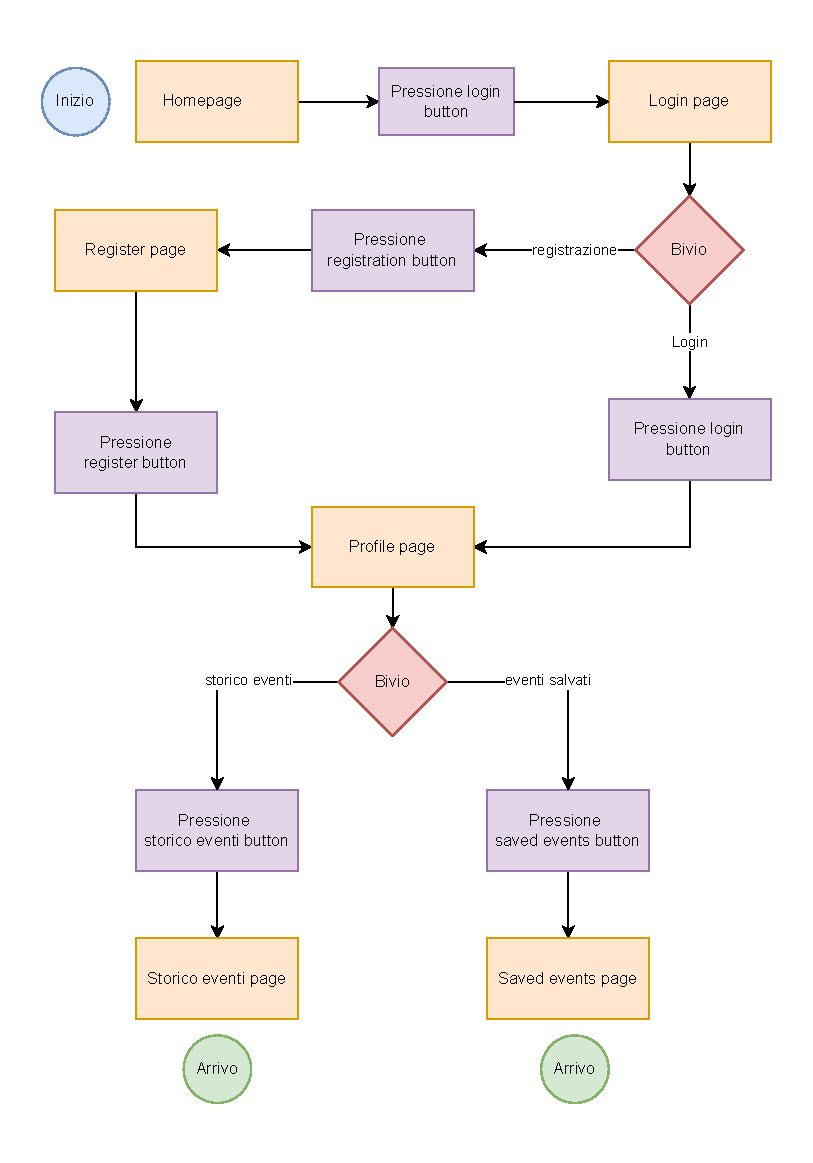
\includegraphics[width=0.7\linewidth]{./images/A1-A2-A3.pdf}
	\caption{Flowchart relativo alle user stories A1, A2 e A3.}
	\label{fig:A1-A2}
\end{figure}

\newpage 

\begin{figure}[!htb]
	\centering
	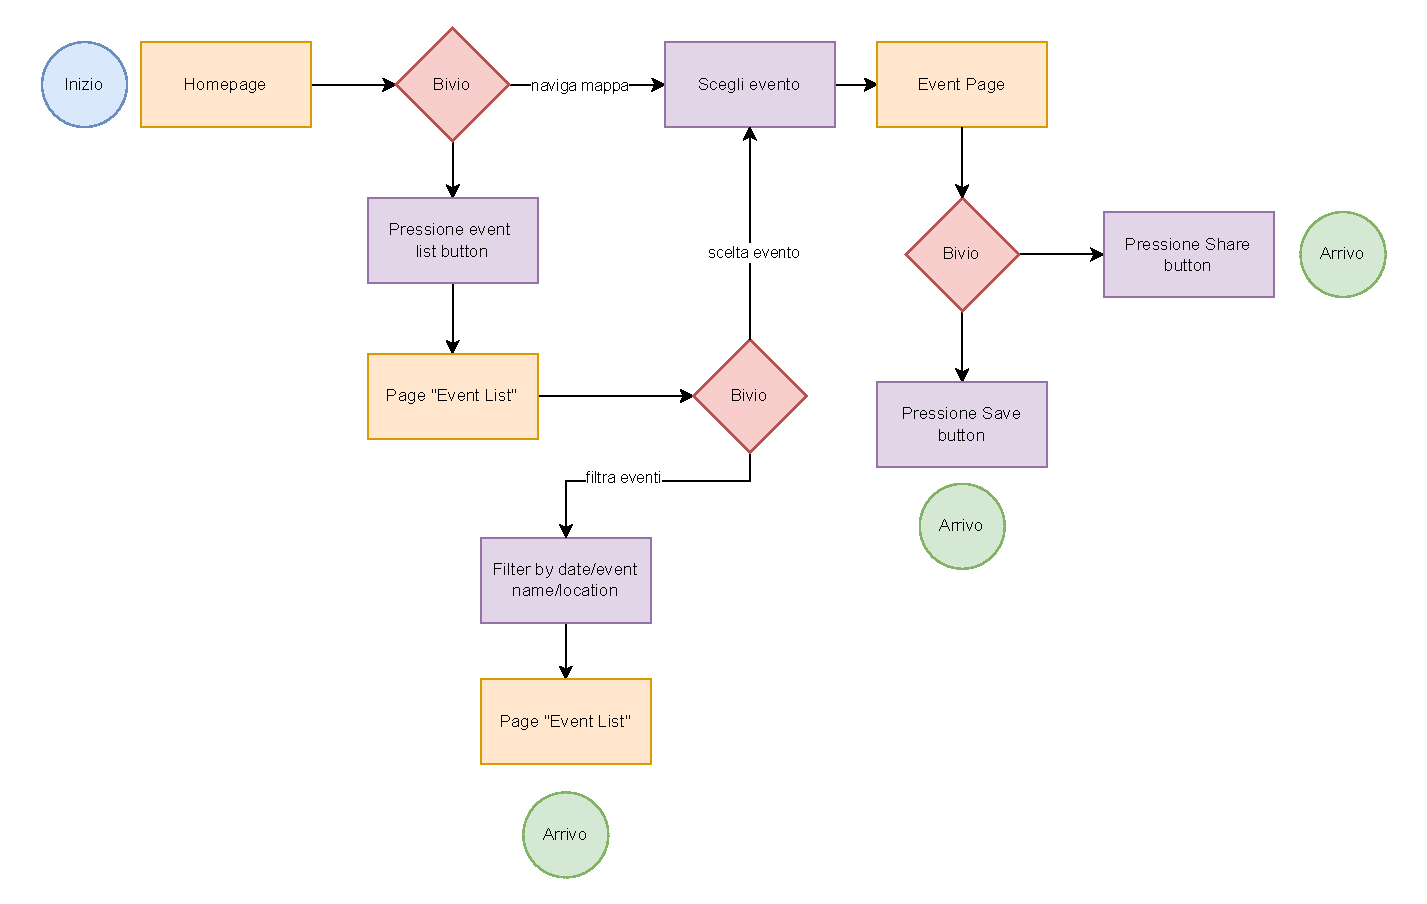
\includegraphics[width=\linewidth]{./images/B1-B2-B4-B8-D1.pdf}
	\caption{Flowchart relativo alle user stories B1, B2, B4, B8 e D1.}
	\label{fig:B1-C1}
\end{figure}


\begin{figure}[!htb]
	\centering
	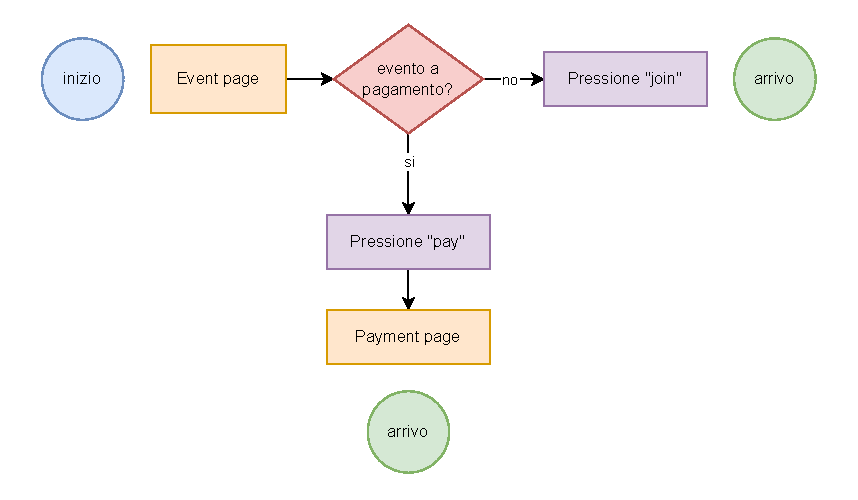
\includegraphics[width=0.8\linewidth]{./images/B5.pdf}
	\caption{Flowchart relativo alla user story B5.}
	\label{fig:B5}
\end{figure}

\newpage  

\begin{figure}[!htb]
	\centering
	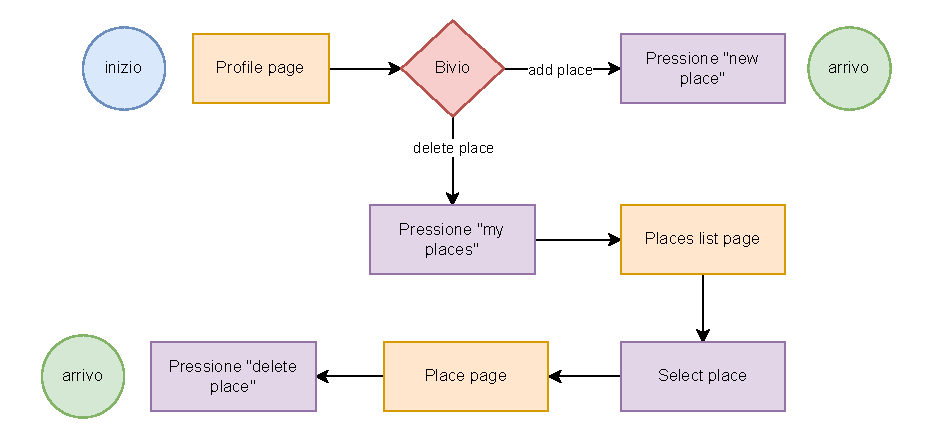
\includegraphics[width=0.8\linewidth]{./images/C1-C2.pdf}
	\caption{Flowchart relativo alle user stories C1 e C2.}
	\label{fig:C1-C2}
\end{figure}

\begin{figure}[!htb]
	\centering
	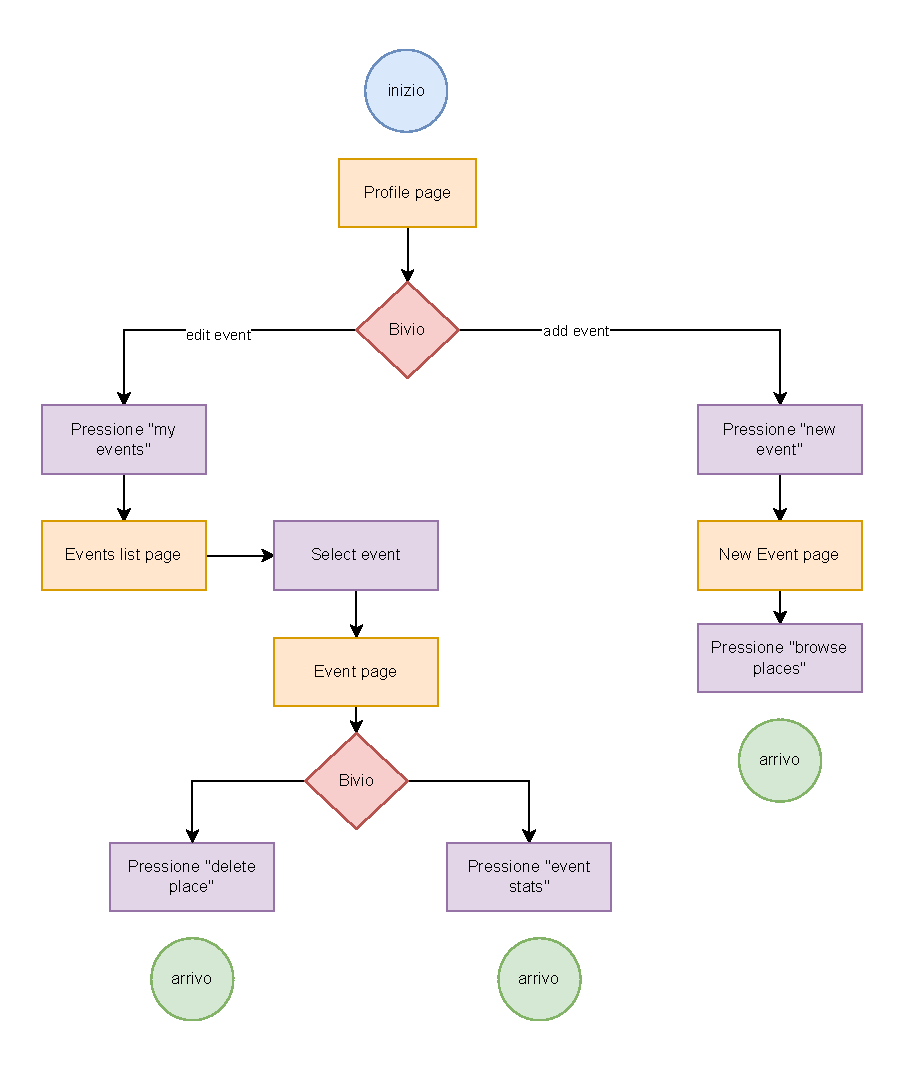
\includegraphics[width=0.8\linewidth]{./images/B3-B6-B7-C3.pdf}
	\caption{Flowchart relativo alle user stories B3, B6, B7 e C3.}
	\label{fig:B3-B6-B7-C3}
\end{figure}

\newpage
\section{Web APIs}

Le API sono state documentate rispettando le specifiche openapi3. La specifica è disponibile nella \href{https://github.com/rtogni00/IS\_Progetto}{repository GitHub}, ed è per comodità riportata di seguito.

\begin{lstlisting}[style=yamlcode, caption={Documentazione API}]
	openapi: 3.0.0
	info:
		version: 1.0.0
		title: "EvenTrento OpenAPI 3.0"
		description: API for managing events.
		license:
		name: MIT
	servers:

		- description: Localhost
		url: http://localhost:8000/api/v1
	
	##################
	# API ENDPOINTS
	##################
	
	paths:
	# path per gestire la registrazione di un utente
	/users/signup:
		post:
			description: >-
				Creates a new user in the system.
			summary: Register a new user
			requestBody:
			required: true
				content:
					application/json:
						schema:
							$ref: '#/components/schemas/User'
			responses:
				"201":
					description: "User created. Link in the Location header"
					headers:
						"Location":
							schema:
								type: string
								description: Link to the newly created student.
				"400":
					description: "Invalid input. Please verify the request body."
				"409":
					description: "User already exists."
				
	# path per gestire il login di un utente gia' registrato
	/users/login:
		post:
			summary: Login to the system
			description: Authenticate the user and return a JWT token.
			requestBody:
				required: true
				content:
					application/json:
						schema:
							type: object
							properties:
								email:
									type: string
									description: "Email address of the user"
								password:
									type: string
									description: "Password for the user account"
							required:
								- email
								- password
			responses:
				'200':
					description: Login successful
					content:
						application/json:
							schema:
								type: object
								properties:
									token:
										type: string
										description: "JWT token to authenticate future requests"
				'400':
					description: Invalid email or password
				'500':
					description: Internal server error
	
	# path per gestire gli eventi salvati dall'utente
	/users/saved-events:
		post:
			summary: Save an event of interest for a user
			description: Allows a user to save an event they are interested in.
			security:
				- bearerAuth: []   # Richiede un token JWT valido per accedere
			requestBody:
				required: true
				content:
					application/json:
						schema:
							type: object
							properties:
								eventId:
									type: integer
									description: The ID of the event to save
								userId:
									type: integer
									description: The ID of the user saving the event
			responses:
				'201':
					description: 'Event saved successfully'
					content:
						application/json:
							schema:
								type: object
								properties:
									message:
										type: string
			'404':
				description: 'Event not found'
			'400':
				description: 'Invalid save request'
			'500':
				description: 'Internal server error'
		get:
			summary: Retrieve saved events for the authenticated user
			description: Returns a list of events saved by the authenticated user.
			security:
				- bearerAuth: []
			responses:
				'200':
					description: 'List of saved events'
					content:
						application/json:
							schema:
								type: array
								items:
									$ref: '#/components/schemas/Event'
			'401':
				description: 'Unauthorized user'
			'500':
				description: 'Internal server error'
				
	# path per creare e fare il retrieving di eventi
	/events:
		get:
			description: Returns a list of events, optionally filtered by date.
			summary: View all events (with optional date filter)
			parameters:
				- in: query
					name: startDate
					schema:
						type: string
						format: date-time
					required: false
			responses:
				'200':
					description: 'Collection of events'
					content:
						application/json:
						schema:
							type: array
							items:
							$ref: '#/components/schemas/Event'
			'400':
				description: 'Invalid date format'
			'500':
				description: 'Internal server error'


	post:
		description: >-
			Creates a new event in the system.
		summary: Create a new event
		security:
			- bearerAuth: []   # Richiede un token JWT valido per accedere
		requestBody:
			required: true
			content:
				application/json:
					schema:
						$ref: '#/components/schemas/EventCreation' # Creating a new event
		responses:
			'201':
				description: 'Event successfully created'
				content:
					application/json:
						schema:
							$ref: '#/components/schemas/Event'  # Returning the created event
		'400':
			description: 'Invalid input, check the event details'
		'403':
			description: 'User not authorized to create an event (only organizers)'
		'500':
			description: 'Internal server error'
					
	# path per la modifica di un evento esistente
	/events/{eventId}:
		put:
			summary: Update an existing event
			description: Allows an organizer to update an event they created.
			security:
				- bearerAuth: []   # Richiede un token JWT valido per accedere
			parameters:
				- in: path
					name: eventId
					schema:
						type: integer
					required: true
					description: The ID of the event to be updated
			requestBody:
				required: true
				content:
					application/json:
						schema:
							$ref: '#/components/schemas/EventUpdate'  # Schema per aggiornamento
			responses:
				'200':
					description: 'Event updated successfully'
					content:
						application/json:
							schema:
								$ref: '#/components/schemas/Event'
			'403':
				description: 'Forbidden. Organizer is not authorized to modify this event.'
			'404':
				description: 'Event not found'
			'500':
				description: 'Internal server error'
				
	# path per l'iscrizione ad un evento                
	/events/{eventId}/registration:
		post:
			summary: Register a participant for an event
			description: Allows a participant to register for a specific event.
			security:
				- bearerAuth: []   # Richiede un token JWT valido per accedere
			parameters:
				- in: path
					name: eventId
					required: true
					schema:
						type: integer
			responses:
				'201':
					description: 'Registration successful'
					content:
						application/json:
							schema:
								type: object
								properties:
									message:
										type: string
			'404':
				description: 'Event not found'
			'400':
				description: 'Invalid registration request'
			'500':
				description: 'Internal server error'
			
	# path per gli spazi
	/places:
		get:
			summary: Retrieve a list of spaces
			description: Returns a list of all available spaces.
			security:
				- bearerAuth: []   # Richiede un token JWT valido per accedere
			responses:
				'200':
					description: 'A list of spaces'
					content:
						application/json:
							schema:
								type: array
								items:
									$ref: '#/components/schemas/Place'
				'500':
					description: 'Internal server error'
					
		post:
			summary: Create a new space
			description: Allows an owner to create a new space for events.
			security:
				- bearerAuth: []   # Richiede un token JWT valido per accedere
			requestBody:
				required: true
				content:
					application/json:
					schema:
						$ref: '#/components/schemas/Place'
			responses:
				'201':
					description: 'Place created successfully'
					content:
						application/json:
							schema:
								$ref: '#/components/schemas/Place'
			'400':
				description: 'Invalid input'
			'500':
				description: 'Internal server error'
				
		put:
			summary: Update an existing space
			description: Allows an owner to update a space they created.
			security:
				- bearerAuth: []   # Richiede un token JWT valido per accedere
			parameters:
				- in: path
					name: spaceId
					required: true
					schema:
						type: integer
			requestBody:
				required: true
				content:
					application/json:
						schema:
							$ref: '#/components/schemas/PlaceUpdate'
			responses:
				'200':
				description: 'Place updated successfully'
				content:
					application/json:
						schema:
							$ref: '#/components/schemas/Place'
			'403':
				description: 'Forbidden. Owner is not authorized to modify this space.'
			'404':
				description: 'Place not found'
			'400':
				description: 'Invalid input'
			'500':
				description: 'Internal server error'
				
	
	#######################
	# COMPONENTS SECTION
	#######################
	
	components:
		schemas:
			User:
				type: object
				required:
					- username
					- email
					- password
					- role
				properties:
					username:
						type: string
						description: "Username of the user"
					email:
						type: string
						description: "Email address of the user"
					password:
						type: string
						description: "Password for the user account"
					role:
						type: string
						enum: [basicUser, owner, organizer]
						description: "Role of the user in the system"
						
			Event:
				type: object
				required:
					- id
					- name
					- date
					- location
					- organizerId
				properties:
					id:
						type: integer
						description: "Unique identifier of the event"
					name:
						type: string
						description: "Name of the event"
					description:
						type: string
						description: "Brief description of the event"
					date:
						type: string
						format: date-time
						description: "Date and time of the event"
					location:
						type: string
						description: "Location where the event will be held"
					organizerId:
						type: integer
						description: "The ID of the organizer who created the event"
			
			EventCreation:
				type: object
				required:
					- name
					- date
					- location
				properties:
					name:
						type: string
						description: "Name of the event"
					description:
						type: string
						description: "Brief description of the event"
					date:
						type: string
						format: date-time
						description: "Date and time of the event"
					location:
						type: string
						description: "Location where the event will be held"
						
			EventUpdate:
				type: object
				required:
				- name
				- description
				- date
				- location
				properties:
					name:
						type: string
						description: "Updated name of the event"
					description:
						type: string
						description: "Updated description of the event"
					date:
						type: string
						format: date-time
						description: "Updated date and time of the event"
					location:
						type: string
						description: "Updated location of the event"
						
			Place: # oggetto per la creazione e la visualizzazione dello spazio
				type: object
				properties:
					id:
						type: integer
						description: Unique identifier of the space
					name:
						type: string
						description: Name of the space
					location:
						type: string
						description: Location of the space
					capacity:
						type: integer
						description: Maximum capacity of the space

   		    PlaceUpdate: # oggetto per l'aggiornamento dello spazio
				type: object
				properties:
					name:
						type: string
						description: Updated name of the space
					location:
						type: string
						description: Updated location of the space
					capacity:
						type: integer
						description: Updated maximum capacity of the space
	
			
		# modalita' di autenticazione che le API utilizzano
		securitySchemes:
			bearerAuth:
				type: http
				scheme: bearer
				bearerFormat: JWT
				
\end{lstlisting}
	

\newpage

\section{Implementation}
\subsection{Repository Implementation}

Il codice del progetto, disponibile su \href{https://github.com/rtogni00/IS_Progetto}{GitHub}, è organizzato secondo il seguente schema:

\begin{lstlisting}[style=treestyle, caption=Struttura della repository]
.
+-- D1
+-- D2
+-- D3
+-- D4
+-- front_end
|   +-- assets // icona della web app
|   +-- index.html
|   +-- pages // html delle varie pagine
|   +-- scripts // codice javascript per la gestione delle varie pagine
+-- node_app
|   +-- app.js // entry point dell'app
|   +-- helperFunctions // funzioni ausiliarie usate durante lo sviluppo
|   +-- .env.example // esempio di file di configurazione delle
|   |                // variabili d'ambiente
|   +-- index.js // aggregatore di supporto ad app.js per maggiore modularita'
|   +-- models // modelli dati mongoose
|   +-- package.json  // file di configurazione del progetto npm
|   +-- package-lock.json
|   +-- routes  // endpoint routes per le APIs
|   +-- tokenChecker.js // middleware per l'autenticazione
|   +-- tests // testing delle funzinalita'
+-- README.md
+-- .gitignore // configurazione git repo
+-- swagger
    +-- evenTrentoAPIs.yaml // documentazione API
\end{lstlisting}


\subsection{Branching strategy e organizzazione del lavoro}

Malgrado i propositi di collaborazione iniziali, verso la fine del mese di
settembre ho preso la decisione di proseguire lo sviluppo in modo individuale.
Come facilmente osservabile dalla commit history del progetto, il contributo
degli altri due membri del gruppo è limitato al processo di brainstorming e
alla realizzazione di alcuni grafici relativi allo User Flow. Tali grafici non
sono presenti nella versione finale del presente documento a causa della loro
modifica nel corso dello sviluppo dell'applicazione.

La branching strategy adottata ha seguito un approccio semplice ma efficace: lo sviluppo è stato incentrato su una
branch principale, garantendo una versione stabile del progetto. Per lo sviluppo di nuove funzionalità o per modifiche significative si è fatto uso di branch temporanee, in modo da non impattare sulla main branch. Una volta completata e testata la nuova funzionalità, questa veniva reinserita nella main branch, e la branch temporanea veniva eliminata. Questo approccio ha garantito il mantenimento di una struttura pulita della repository, consentendo al contempo uno sviluppo "risk-free" dell'applicazione.


Una descrizione dettagliata delle statistiche di sviluppo è riportata in Figura \ref{fig:commits}. Come raffigurato nei grafici, lo sviluppo ha avuto un forte picco nel corso del mese di ottobre, durante
il quale è stata svolta buona parte dell'attività di progettazione. Dopodiché si è continuato ad un regime pressoché costante nei mesi di novembre, dicembre e gennaio, con la conclusione del progetto durante la prima settimana di febbraio.

\newpage


%\begin{verbatim}
%git log --format='%aN <%aE>' | sort | uniq -c | sort -nr
%\end{verbatim}

\begin{figure}[!htb]
	\centering
	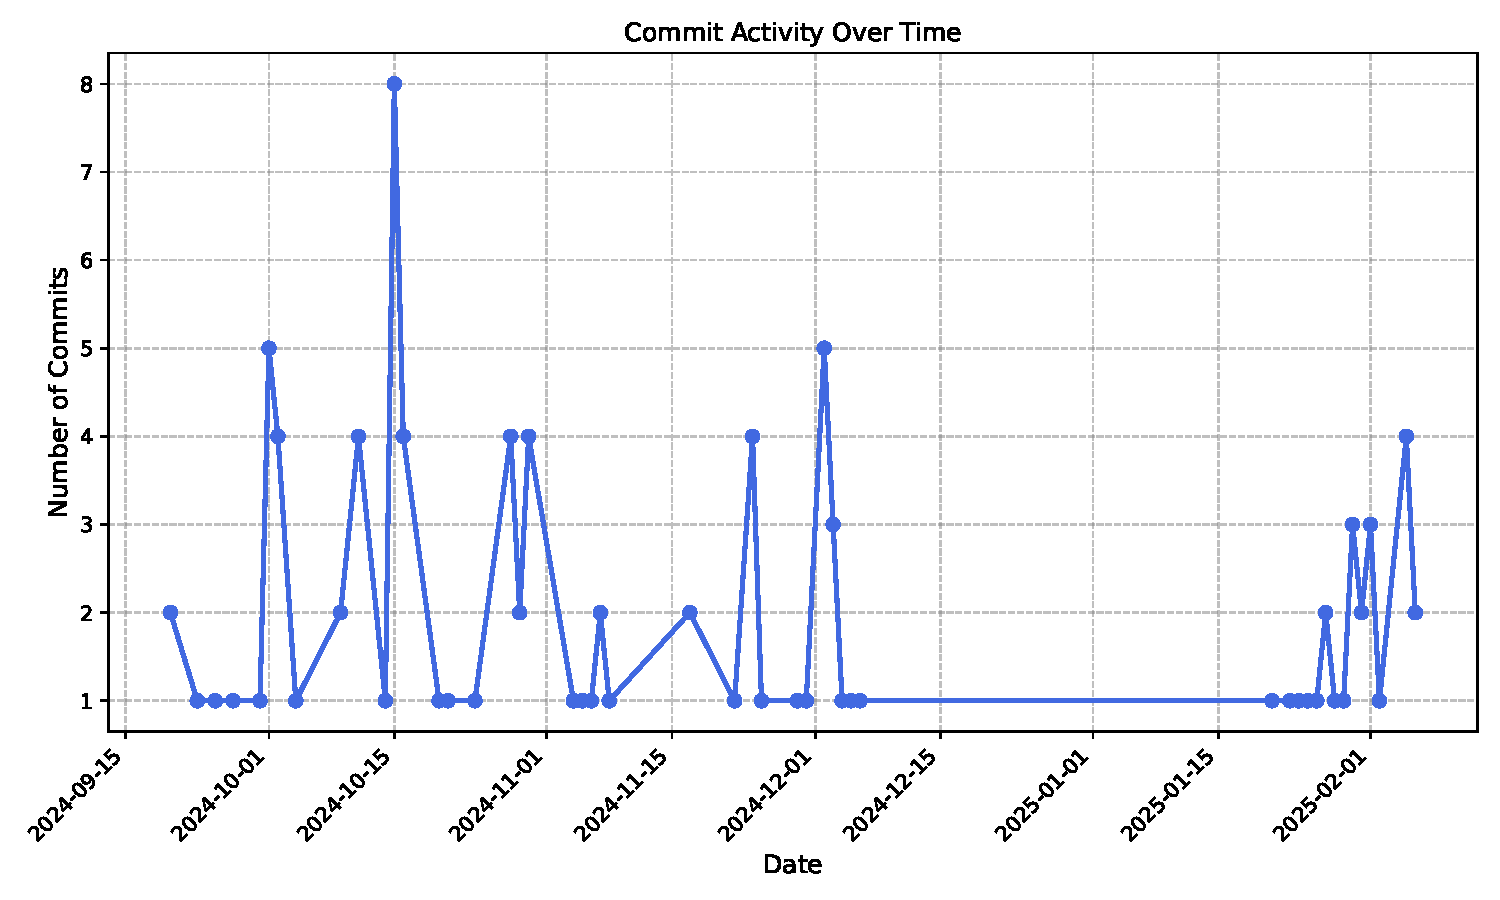
\includegraphics[width=0.9\linewidth]{./images/commitsOverTime.pdf}
	\smallskip
%	\caption{Grafico rappresentante i commit durante il periodo di sviluppo.}
%	\label{fig:commits}
%\end{figure}
%
%\begin{figure}[!htb]
%	\centering
	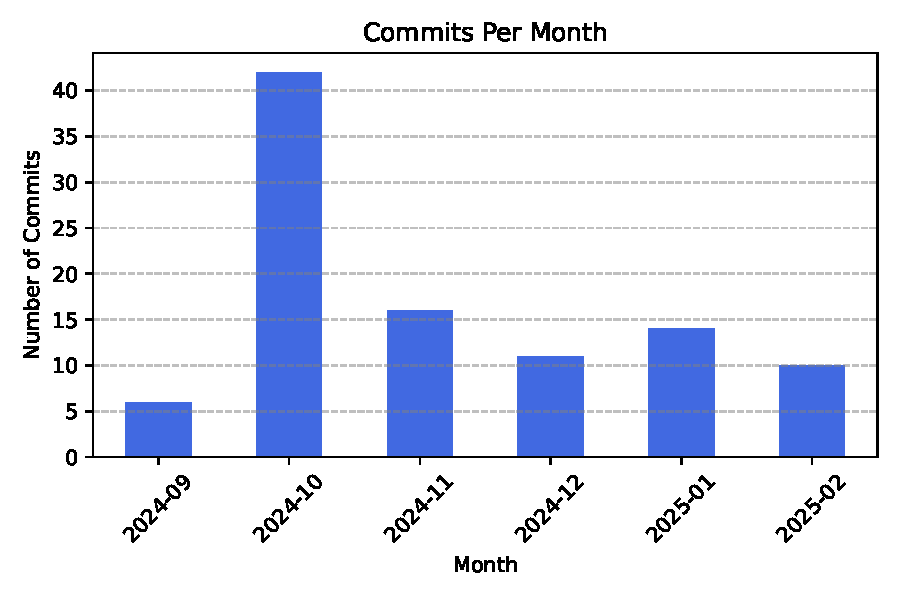
\includegraphics[width=0.6\linewidth]{./images/barPlot.pdf}
	\vskip .5cm
%	\caption{Grafico rappresentante i commit durante il periodo di sviluppo.}
%	\label{fig:barPlot}
%\end{figure}
%
%\begin{figure}[!htb]
%	\centering
	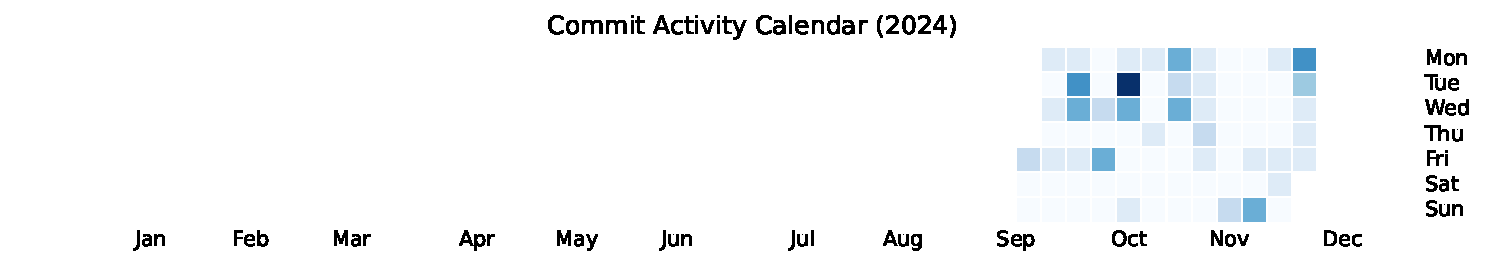
\includegraphics[width=\linewidth]{./images/calendar24.pdf}

	\vskip .5cm
	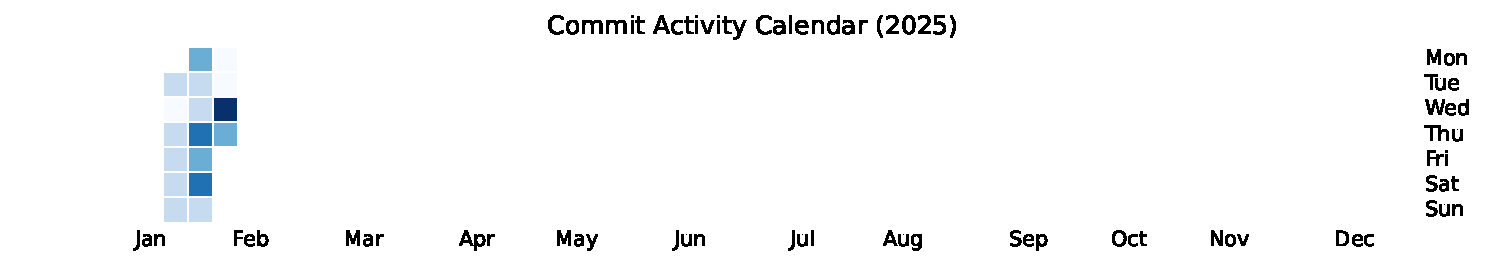
\includegraphics[width=\linewidth]{./images/calendar25.pdf}
	\caption{Grafici rappresentanti la distribuzione del lavoro durante il periodo di sviluppo.}
	\label{fig:commits}
\end{figure}
\newpage


\subsection{Dependencies}

Il progetto npm fa uso dei seguenti moduli:
\begin{itemize}
    \item \textbf{Cors} per il supporto alle chiamate cross-origin;
    \item \textbf{Express} come framework per il backend;
    \item \textbf{Jsonwebtoken} per gestire l'autenticazione;
    \item \textbf{Mongoose} per interfacciarsi con mongoDB;
    \item \textbf{Axios} per interagire con l'API di \href{https://www.openstreetmap.org/#map=6/42.09/12.56}{OpenStreetMap};
    \item \textbf{Bcrypt} per la gestione delle password.
\end{itemize}

Sono inoltre riportate le seguenti dipendenze di sviluppo:
\begin{itemize}
    \item \textbf{Dotenv} per la gestione delle variabili d'ambiente;
    \item \textbf{Jest} per il testing;
    \item \textbf{Supertest} per il testing della endpoint express.
\end{itemize}

\subsection{Database}

La gestione dei dati è stata realizzata basandosi su un database non
relazionale. In particolare, si è fatto uso del servizio offerto da
\href{https://www.mongodb.com/products/platform/atlas-database}{Atlas MongoDB}.

Per la gestione dei dati necessari per il funzionamento dell'applicazione sono state definite tre strutture dati mediante Mongoose:
\begin{itemize}
	\item \textbf{Event}: per gestire tutte le funzionalità legate alla creazione, modifica ed eliminazione degli eventi, nonché all'interazione tra users ed eventi;
%	\item \textbf{EventRegistration}: per gestire correttamente l'iscrizione e la disiscrizione degli utenti dagli eventi;
	\item \textbf{Place}: per gestire tutte le funzionalità legate alla creazione, modifica ed elimazione dei luoghi;
	\item \textbf{User}: per gestire le tre tipologie di utente e le attività ad esse collegate.
\end{itemize}

\newpage
\subsection{Testing}

Le API sono state testate tramite una test-suite sviluppata mediante l'utilizzo di \href{https://jestjs.io/}{Jest}. L’implementazione dei test è organizzata in file \verb|.test.js| situati all'interno della cartella \verb*|tests|. Ogni file contiene tutti i test case relativi ad una determinata route.


\begin{table}[!htb]
	\centering
	\renewcommand{\arraystretch}{1.7} % Adjust row height
	\setlength{\tabcolsep}{6pt} % Adjust column spacing
	\resizebox{\textwidth}{!}
	{%
	\begin{tabular}{p{.4cm} p{3.5cm} p{2.5cm} p{2.5cm} p{5cm} p{1.5cm}}
		\toprule
		\rowcolor{gray!20}
		\# & Descrizione & Test Data & Precondizioni & Risultato Atteso & Risultato Effettivo \\ \midrule
		1 & Fetching di tutti gli eventi                                                 &                                                               &                                             & Viene ritornato un array contenente tutti gli eventi presenti nel database                                     & Risultato atteso      \\\midrule
		2 & Fetching degli eventi filtrando per nome                                     & Titolo dell'evento                                            &                                             & Viene ritornato un array contenente gli eventi che corrispondono con i filtri di ricerca (possibilmente vuoto) & Risultato atteso      \\\midrule
		3 & Fetching degli eventi filtrando per location                                 & Luogo dell'evento                                             &                                             & Viene ritornato un array contenente gli eventi che corrispondono con i filtri di ricerca (possibilmente vuoto) & Risultato atteso      \\\midrule
		4 & Fetching degli eventi filtrando per data                                     & Data dell'evento                                              &                                             & Viene ritornato un array contenente gli eventi che corrispondono con i filtri di ricerca (possibilmente vuoto) & Risultato atteso      \\\midrule
		5 & Creazione di un nuovo evento con dati validi                                 & Dati dell'evento che si vuole creare, token di autenticazione & Login effettuato con un profilo "organizer" & Viene creato un evento con i dati specificati                                                                  & Risultato atteso      \\\midrule
		5.1 & Creazione di un nuovo evento senza essere loggati                            & Dati dell'evento che si vuole creare                          & Login non effettuato                        & Viene mostrato un messaggio di errore e l'evento non viene creato                                              & Risultato atteso      \\\midrule
		5.2 & Creazione di un nuovo evento essendo loggati con un profilo non  "organizer" & Dati dell'evento che si vuole creare, token di autenticazione &                                             & Viene mostrato un messaggio di errore e l'evento non viene creato                                              & Risultato atteso      \\ \midrule
		6 &  Registrazione di un nuovo utente inserendo tutti i dati & Dati dell'utente che si vuole registrare & Utente non precedentemente registrato & Viene creato un nuovo User nel database & Risultato atteso \\\midrule
		6.1 &  Registrazione di un nuovo utente con dati mancanti & Dati parziali dell'utente che si vuole registrare & Utente non precedentemente registrato & Viene mostrato un messaggio di errore e l'utente non viene registrato & Risultato atteso \\\midrule
		6.2 &  Registrazione di un nuovo utente con email già in uso & Dati dell'utente che si vuole registrare & Utente non precedentemente registrato & Viene mostrato un messaggio di errore e l'utente non viene registrato & Risultato atteso \\\midrule
		6.3 &  Registrazione di un nuovo utente con username già in uso & Dati dell'utente che si vuole registrare & Utente non precedentemente registrato & Viene mostrato un messaggio di errore e l'utente non viene registrato & Risultato atteso \\\midrule
		7 &  Autenticazione con dati corretti & Email e password corretti & Utente precedentemente registrato & L'utente viene loggato nel sistema e può accedere alla propria area personale & Risultato atteso \\\midrule
		7.1 &  Autenticazione con password errata  & Email corretta, password errata & Utente precedentemente registrato & Viene mostrato un messaggio di errore e l'utente viene reindirizzato alla pagina di login & Risultato atteso \\\midrule
		7.2 &  Autenticazione con email errata  & Email errata, password corretta & Utente precedentemente registrato & Viene mostrato un messaggio di errore e l'utente viene reindirizzato alla pagina di login & Risultato atteso \\\midrule
		7.3 &  Autenticazione senza fornire dati  &  & Utente precedentemente registrato & Viene mostrato un messaggio di errore e l'utente viene reindirizzato alla pagina di login & Risultato atteso \\\midrule		
	\end{tabular}
}

\end{table}

\newpage

\begin{table}[!htb]
	\centering
	\renewcommand{\arraystretch}{1.7} % Adjust row height
	\setlength{\tabcolsep}{6pt} % Adjust column spacing
	\resizebox{\textwidth}{!}
	{%
	\begin{tabular}{p{.5cm} p{3.5cm} p{2.5cm} p{2.5cm} p{5cm} p{1.5cm}}
	\toprule
	8 & Fetching delle location &  & Location presenti nel database & Viene ritornato un array contenente tutte le location presenti nel database & Risultato atteso \\\midrule
	8.1 & Fetching delle location senza essere loggati &  & Utente non autenticato & L'operazione non è permessa, viene ritornato un messaggio di errore & Risultato atteso \\\midrule
	8.2 & Fetching delle location con un profilo diverso da "organizer" &  & Utente autenticato con ruolo "user" o "owner" & L'operazione non è permessa, viene ritornato un messaggio di errore & Risultato atteso \\\midrule
	9 & Fetching di una location in base al nome & Nome della location valido & Database contenente almeno una location con quel nome & Viene ritornato l'oggetto della location corrispondente al nome fornito & Risultato atteso \\\midrule
	9.1 & Fetching di una location in base al nome senza essere loggati & Nome della location valido & Utente non autenticato & L'operazione non è permessa, viene ritornato un messaggio di errore& Risultato atteso \\\midrule
	9.2 & Fetching di una location in base al nome con un profilo diverso da "organizer" & Nome della location valido & Utente autenticato con ruolo "user" o "owner" & L'operazione non è permessa, viene ritornato un messaggio di errore & Risultato atteso \\\midrule
	10 & Creazione di una location & Dati relativi alla location & Utente autenticato con ruolo "owner" & La nuova location viene creata nel database e restituita nella risposta & Risultato atteso \\\midrule
	10.1 & Creazione di una location senza essere loggati & Dati relativi alla location & Utente non autenticato & L'operazione non è permessa, viene ritornato un messaggio di errore e la location non viene creata & Risultato atteso \\\midrule
	10.2 & Creazione di una location con un profilo diverso da "owner" & Dati relativi alla location & Utente autenticato con ruolo "user" o "organizer" & L'operazione non è permessa, viene ritornato un messaggio di errore e la location non viene creata & Risultato atteso \\\midrule
	10.3 & Creazione di una location senza inserire tutti i dati necessari & Dati parziali (e.g., solo nome) & Utente autenticato con ruolo "owner" & Viene ritornato un messaggio di errore e la location non viene creata & Risultato atteso \\\bottomrule
	
	\end{tabular}
}
\caption{Test case implementati per testare le funzionalità implementate. I dati a cui si fa riferimento nella colonna "Test Data" sono quelli riportati nei Listing \ref{lst:events}, \ref{lst:users}, e \ref{lst:places}.}
\end{table}

Di seguito sono riportati per completezza i modelli relativi agli eventi, agli utenti, e ai luoghi.

\begin{lstlisting}[style=jscode, caption={Modello per gli eventi.}, label={lst:events}]
	var mongoose = require('mongoose');
	var Schema = mongoose.Schema;
	
	const EventSchema = new Schema({
		name: {
			type: String,
			required: true,
			description: "Name of the event"
		},
		description: {
			type: String,
			description: "Description of the event"
		},
		date: {
			type: Date,
			required: true,
			description: "Date and time of the event"
		},
		location: {
			type: String,
			required: true,
			description: "Location of the event"
		},
		latitude: { 
			type: Number, 
			description: "Latitude of the location" 
		},
		longitude: { 
			type: Number,
			description: "Longitude of the location" 
		},
		capacity: {
			type: Number,
			required: true,
			description: "Maximum number of participants"
		},
		organizer: {
			type: String,
			ref: 'User',
			required: true,
			description: "Reference to the organizer who created the event"
		},
		pictures: {
			type: [String], // Array of strings for picture URLs
			description: "Array of picture URLs of the event location"
		},
		participants: {
			type: Number,
			default: 0,
			description: "Current number of participants"
		},
		enrolledUsers: {
			type: [Schema.Types.ObjectId], // Array of user IDs
			ref: 'User',
			description: "Array of user IDs representing enrolled users"
		}
	}, {
		timestamps: true
	});
	
	// Create and export the Event model
	const EventModel = mongoose.model('Event', EventSchema);
	module.exports = EventModel;
\end{lstlisting}


\begin{lstlisting}[style=jscode, caption={Modello per gli user.}, label={lst:users}]
	const mongoose = require('mongoose');
	const Schema = mongoose.Schema;
	
	// Define the user schema
	const UserSchema = new Schema({
		username: {
			type: String,
			required: true,
			unique: true
		},
		email: {
			type: String,
			required: true,
			unique: true
		},
		password: {
			type: String,
			required: true
		},
		role: {
			type: String,
			enum: ['user', 'owner', 'organizer'], // user = basicUser
			required: true
		},
		
		// Array of saved event IDs
		savedEvents: [{
			type: mongoose.Schema.Types.ObjectId,
			ref: 'Event'
		}],
		
		// Array of past events (event history)
		pastEvents: [{
			type: mongoose.Schema.Types.ObjectId,
			ref: 'Event'
		}]
	}, { timestamps: true });
	
	// Create and export the User model
	const UserModel = mongoose.model('User', UserSchema);
	module.exports = UserModel;
\end{lstlisting}

\begin{lstlisting}[style=jscode, caption={Modello per i luoghi.}, label={lst:places}]
	var mongoose = require('mongoose');
	var Schema = mongoose.Schema;
	
	// Define the place schema
	const PlaceSchema = new Schema({
		name: {
			type: String,
			required: true
		},
		location: {
			type: String,
			required: true
		},
		capacity: {
			type: Number,
			required: true
		},
		owner: {
			type: String,
			required: true
		}
	}, { timestamps: true });
	
	// Create and export the Place model
	const PlaceModel = mongoose.model('Place', PlaceSchema);
	module.exports = PlaceModel;
\end{lstlisting}
	
\section{Front-End}

Trattandosi di un "solo Dev project", non è stato possibile implementare tutte le funzionalità inizialmente pianificate. A causa di tale limitazione, ho preso la decisione di dedicare la maggior parte del tempo alla progettazione e allo sviluppo della backend. Il risultato è una backend completa, che offre tutte le API necessarie per lo sviluppo di una front-end funzionale. La parte di front-end effettivamente realizzata ruota invece intorno alle funzionalità offerte alla categoria di utenti "BasicUser".

In particolare, l'applicazione consta di una Home Page, di una pagina per la gestione del profilo personale, di una pagaina per il browsing degli eventi e di una pagina per la visualizzazione dei dettagli di un evento\footnote{Gli screenshot riportati sono stati effettuati utilizzando un laptop. L'intero front-end è tuttavia realizzato in modo tale da risultare totalmente compatibile con i dispositivi mobile.}.

\begin{figure}[!htb]
	\centering
	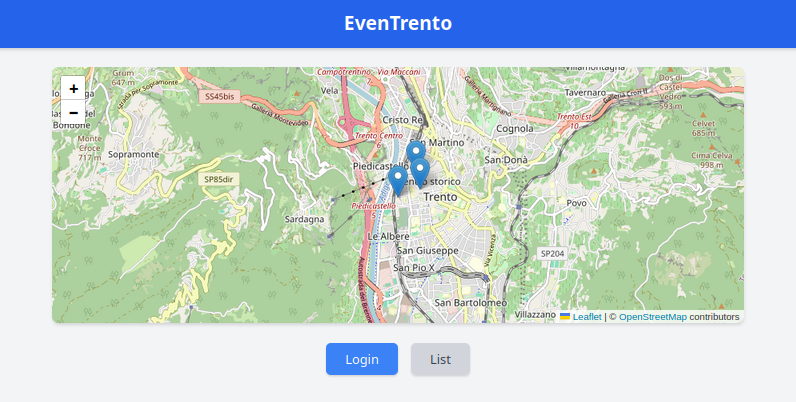
\includegraphics[width=0.8\linewidth]{./images/Index.png}
	\caption{Pagina principale dell'applicazione.}
	\label{fig:index}
\end{figure}
\newpage

In Figura \ref{fig:index} è rappresentata la pagina principale dell'applicazione. Da qui è possibile esplorare la mappa, visualizzare la lista degli eventi o effettuare il login.

\begin{figure}[!htb]
	\centering
	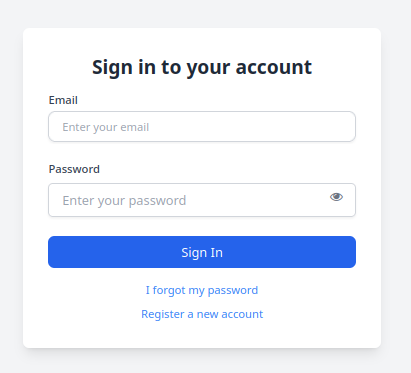
\includegraphics[width=0.5\linewidth]{./images/Login.png}
	\caption{Pagina di login.}
		\label{fig:login}
\end{figure}

Qualora l'utente sia già in possesso di un profilo, a seguito del login viene mostrata una versione della Home Page aggiornata con un bottone per raggiungere la propria area personale (vedi Figura \ref{fig:mainPageAfterLogin}). Alternativamente, dalla pagina di login mostrata in Figura \ref{fig:login} è possibile raggiungere il modulo per la registrazione di un nuovo utente (vedi Figura \ref{fig:registration}).


\begin{figure}[!htb]
	\centering
	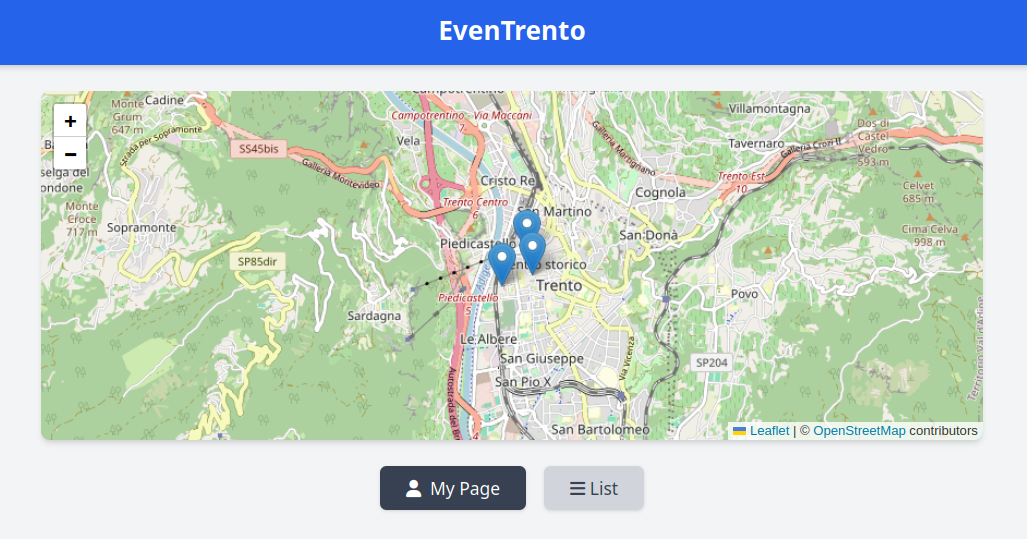
\includegraphics[width=0.9\linewidth]{./images/mainPageAfterLogin.png}
	\caption{Pagina principale dell'applicazione a seguito del login.}
	\label{fig:mainPageAfterLogin}
\end{figure}

\newpage

\begin{figure}[!htb]
	\centering
	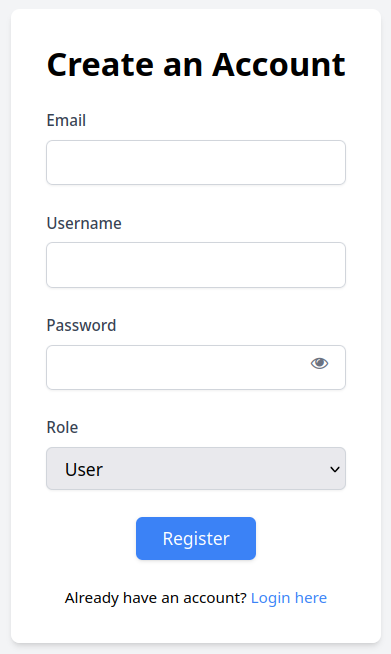
\includegraphics[width=0.3\linewidth]{./images/Registration.png}
	\caption{Pagina di registrazione.}
	\label{fig:registration}
\end{figure}


\begin{figure}[htb]
	\centering
	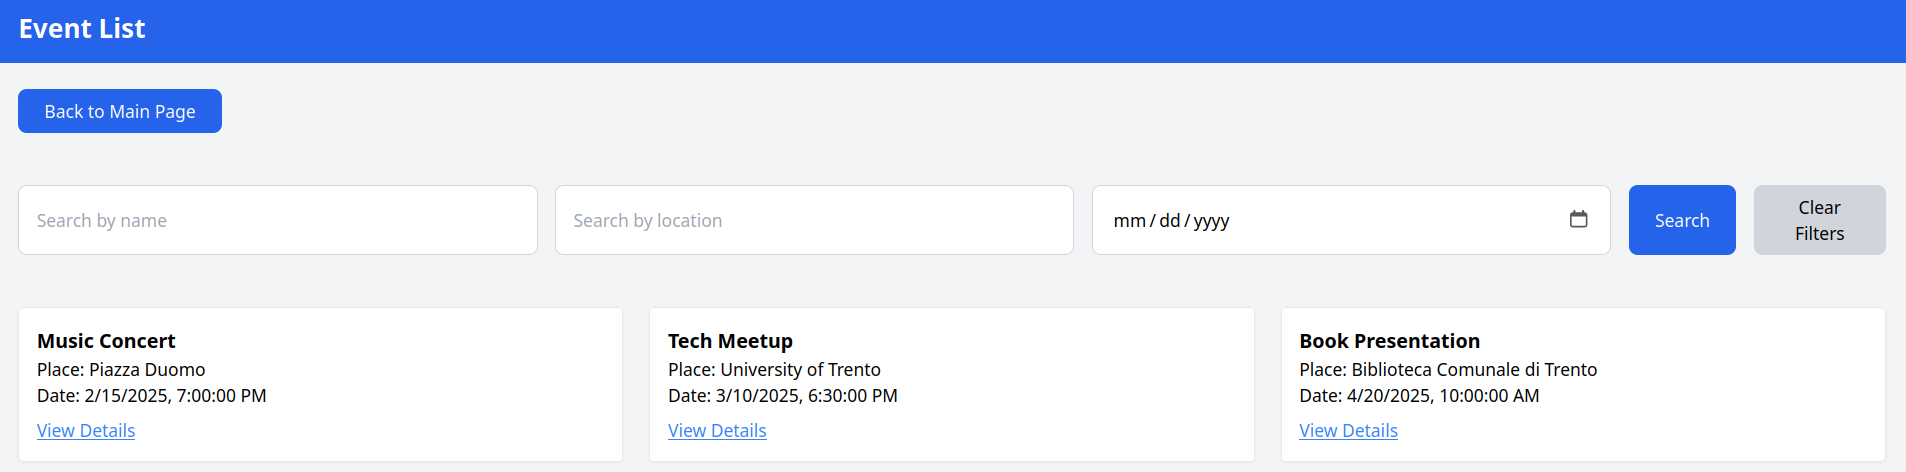
\includegraphics[width=\textwidth]{./images/EventList.png} % Adjust width as needed
	\vskip .5cm
	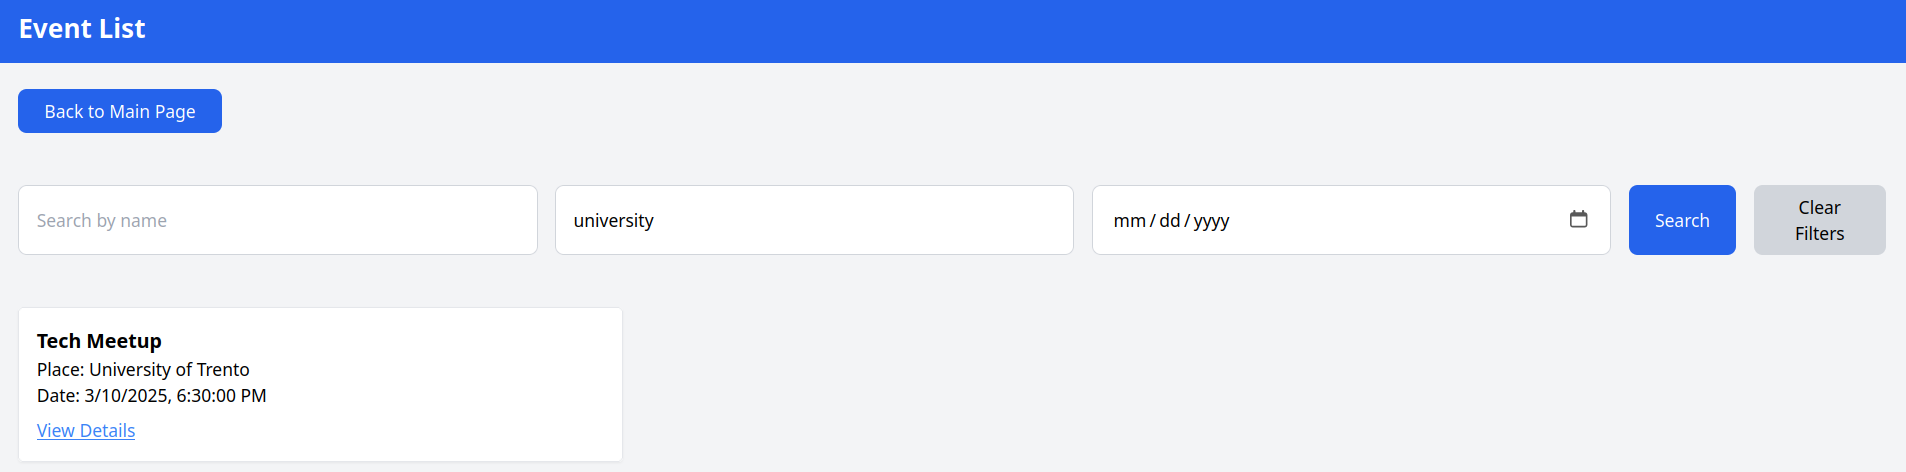
\includegraphics[width=\textwidth]{./images/EventListFilter.png} % Adjust width as needed
	\caption{Top: lista degli eventi senza filtri. Bottom: lista degli eventi filtrando per location.}
	\label{fig:eventList}
\end{figure}




In Figura \ref{fig:eventList} è mostrata la lista degli eventi disponibili. Come mostrato nella parte inferiore della figura, è possibile filtrare gli eventi per nome, location e data. Una volta selezionato un evento, si apre una pagina contenente la descrizione dettagliata dello stesso, come mostrato in Figura \ref{fig:eventDetails1}. I pulsanti "Enroll" e "Save Event" consentono di interagire con l'evento in questione, e vengono aggiornati dinamicamente a seconda dello stato corrente del sistema (vedi Figure \ref{fig:eventDetails1}, \ref{fig:eventDetails2} e \ref{fig:eventDetails3}).

\newpage

\begin{figure}[!htb]
	\centering
	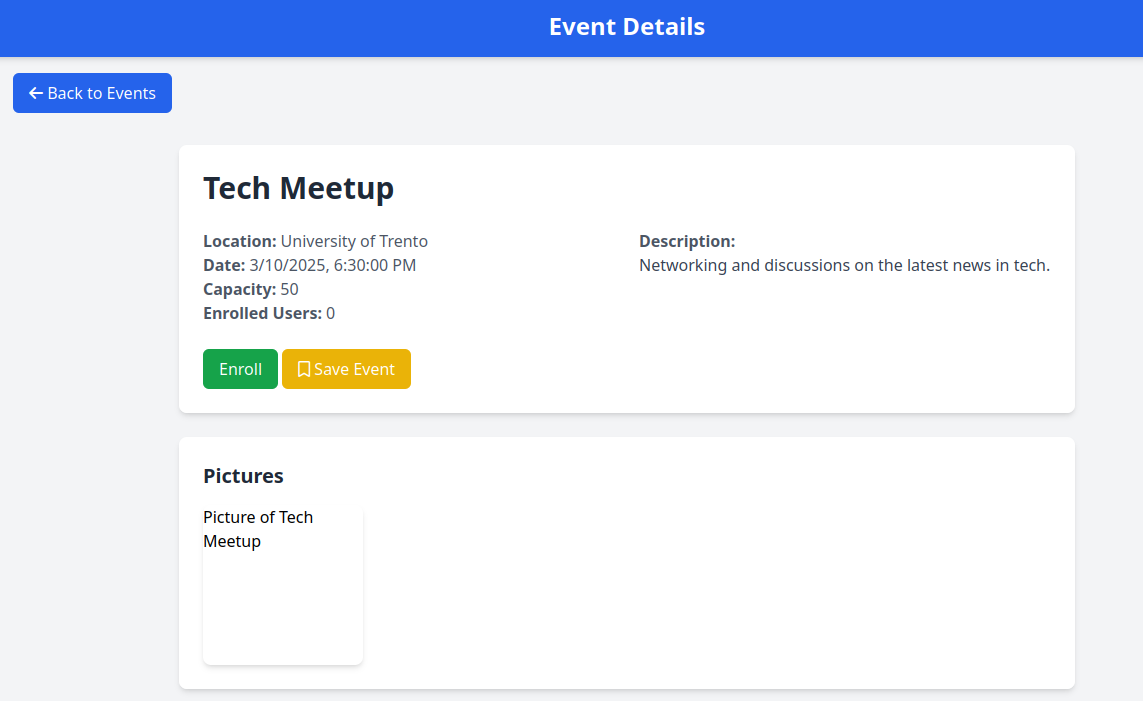
\includegraphics[width=0.9\linewidth]{./images/EventDetails1.png}
	\caption{Pagina dettagli evento.}
	\label{fig:eventDetails1}
\end{figure}

\begin{figure}[!htb]
	\centering
	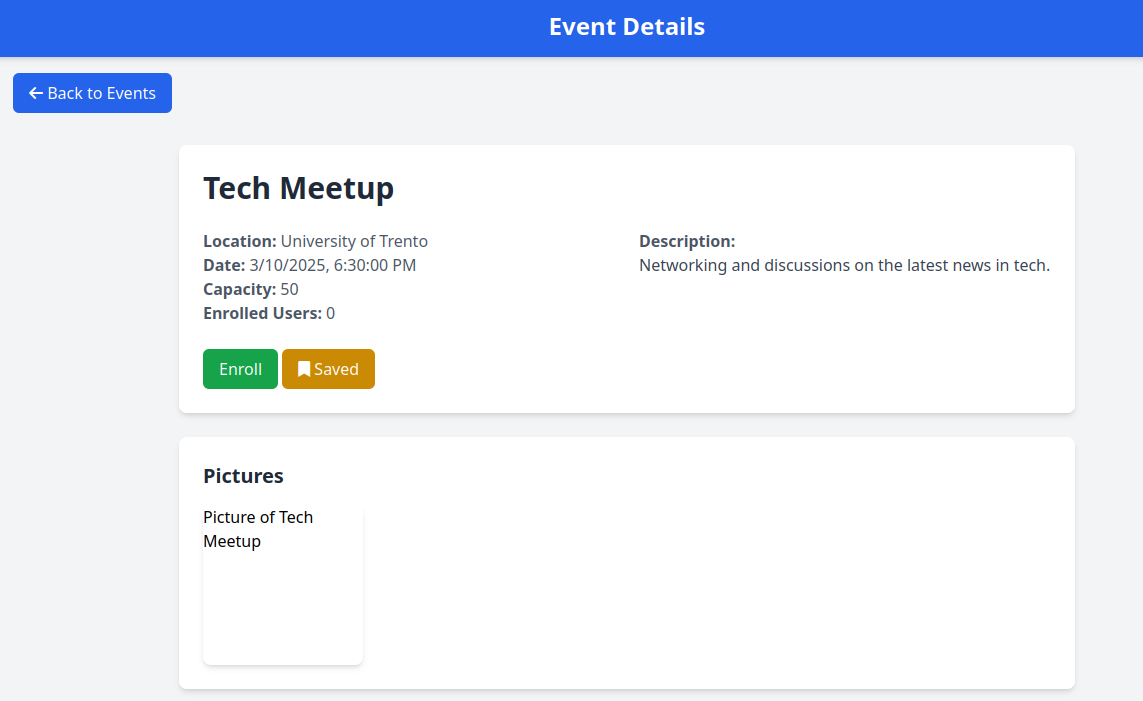
\includegraphics[width=0.9\linewidth]{./images/EventDetails2.png}
	\caption{Pagina dettagli evento salvato dallo user.}
	\label{fig:eventDetails2}
\end{figure}

\newpage

\begin{figure}[!htb]
	\centering
	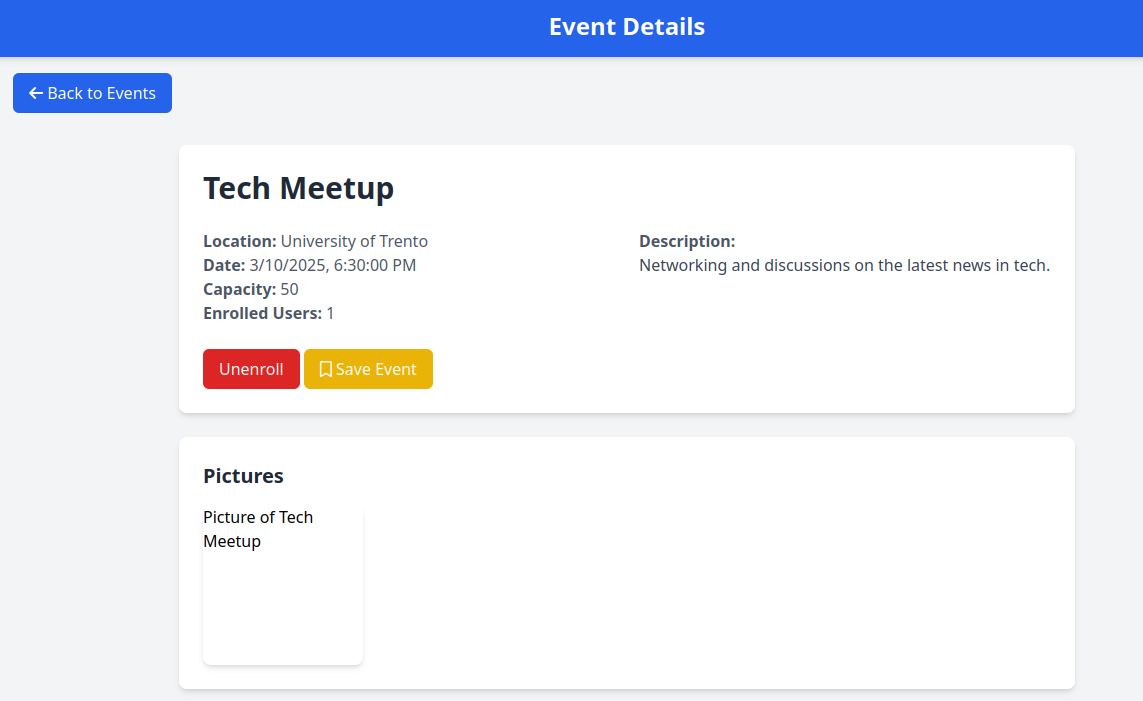
\includegraphics[width=0.9\linewidth]{./images/EventDetails3.png}
	\caption{Pagina dettagli evento a cui lo user è iscritto.}
	\label{fig:eventDetails3}
\end{figure}

In Figura \ref{fig:profile} è invece mostrato il profilo personale. Da qui l'utente può cambiare la password, effettuare il logout, e gestire gli eventi salvati e a cui è iscritto.

\begin{figure}[!htb]
	\centering
	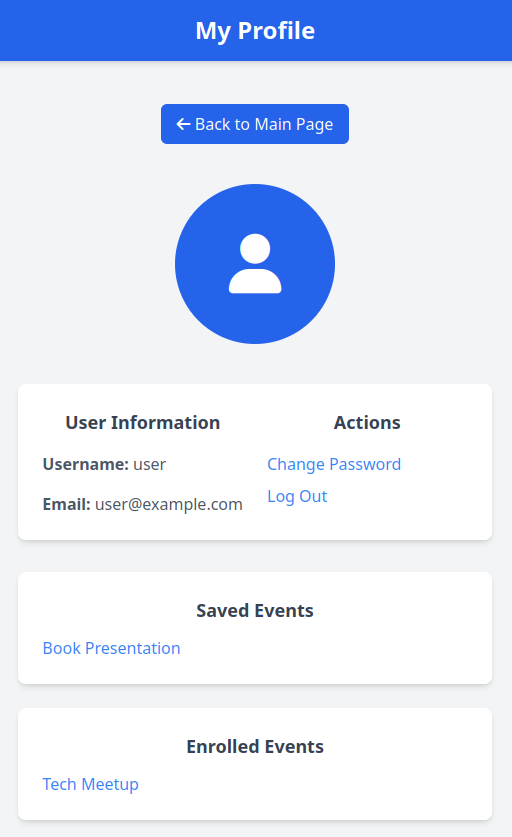
\includegraphics[width=0.4\linewidth]{./images/Profile.png}
	\hspace{1cm}
	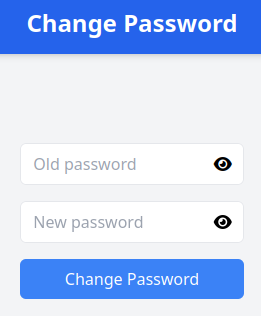
\includegraphics[width=0.25\linewidth]{./images/changePwd.png}
	\caption{Profilo personale dello user (sx), modulo per il cambio password (dx).}
	\label{fig:profile}
\end{figure}
\newpage

\section{Deployment}

Per il deployment è stata utilizzata la piattaforma \href{https://render.com/}{Render.com}. Il \href{https://is-progetto-1.onrender.com}{frontend} e il \href{https://is-progetto.onrender.com}{backend} sono deployati separatamente, ma si appoggiano alla stessa repository GitHub.

Per problemi con il deploy contattare \href{mailto:roberto.togni-1@studenti.unitn.it}{roberto.togni-1@studenti.unitn.it}.

	
\end{document}
